\subsection{Reguladores de voltaje}

El sistema emplea dos reguladores DC-DC step-down para adaptar la tensión de alimentación principal (24V DC) a los niveles requeridos por diferentes subsistemas:

\underline{Regulador 24V - 5V:} Regulador conmutado step-down con capacidad de 5 A. Este regulador alimenta:
\begin{itemize}[label=$\bullet$]
\item Arduino Mega 2560 (consumo típico 0.35 A, picos de 0.5 A)
\item Raspberry Pi 5 (consumo típico 3 A, picos de 4 A)
\item Cámara USB (consumo típico 0.5 A)
\end{itemize}

La capacidad total requerida es de 5 A en condiciones de pico, considerando operación simultánea de todos los dispositivos a carga máxima. El regulador seleccionado proporciona exactamente esta capacidad. Este consumo equivale a 0.89 A en operación normal y 1.16 A en pico desde el lado de 24V (considerando eficiencia del 90\%), como se detalla en la Tabla \ref{tab:consumo_energetico}.

\underline{Regulador 24V - 12V:} Regulador conmutado step-down con capacidad de 10 A. Este regulador alimenta:
\begin{itemize}[label=$\bullet$]
    \item Dos servomotores Dynamixel MX-106T/R (consumo máximo de 4.8 A cada uno)
    \item Circuitos lógicos de drivers de motores (aproximadamente 100 mA por driver)
\end{itemize}

El consumo total en el lado de 12V es de 9.9 A en condiciones de pico (operación simultánea de ambos servos bajo carga), lo que equivale a 5.5 A en el lado de 24V (considerando eficiencia del 90\%), como se detalla en la Tabla \ref{tab:consumo_energetico}. El regulador de 10 A proporciona margen de seguridad del 1\% en el lado de 12V para picos transitorios.

La Figura \ref{fig:diagrama_voltajes} ilustra el esquema completo de distribución de voltajes desde la fuente primaria de 24V hasta todos los componentes del sistema.

\begin{figure}[H]
\centering
% TODO: Agregar imagen del diagrama de distribución de voltajes
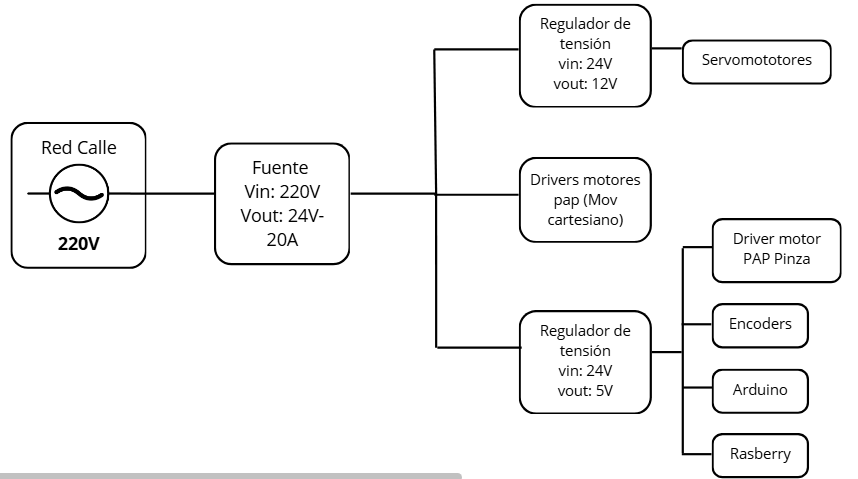
\includegraphics[width=0.75\textwidth]{img/diagrama_voltajes_real.png}
\caption{\textit{Diagrama de distribución de voltajes del sistema mostrando fuente de 24V, reguladores step-down (24V→5V y 24V→12V), y conexiones a todos los componentes}}
\label{fig:diagrama_voltajes}
\end{figure}
